% !TeX program = pdfLaTeX
\documentclass[12pt]{article}
\usepackage{amsmath}
\usepackage{graphicx,psfrag,epsf}
\usepackage{enumerate}
\usepackage{natbib}
\usepackage{textcomp}
\usepackage[hyphens]{url} % not crucial - just used below for the URL
\usepackage{hyperref}
\providecommand{\tightlist}{%
  \setlength{\itemsep}{0pt}\setlength{\parskip}{0pt}}

%\pdfminorversion=4
% NOTE: To produce blinded version, replace "0" with "1" below.
\newcommand{\blind}{0}

% DON'T change margins - should be 1 inch all around.
\addtolength{\oddsidemargin}{-.5in}%
\addtolength{\evensidemargin}{-.5in}%
\addtolength{\textwidth}{1in}%
\addtolength{\textheight}{1.3in}%
\addtolength{\topmargin}{-.8in}%

%% load any required packages here



% Pandoc citation processing

\usepackage{booktabs}
\usepackage{longtable}
\usepackage{array}
\usepackage{multirow}
\usepackage{wrapfig}
\usepackage{float}
\usepackage{colortbl}
\usepackage{pdflscape}
\usepackage{tabu}
\usepackage{threeparttable}
\usepackage{threeparttablex}
\usepackage[normalem]{ulem}
\usepackage{makecell}
\usepackage{xcolor}

\begin{document}


\def\spacingset#1{\renewcommand{\baselinestretch}%
{#1}\small\normalsize} \spacingset{1}


%%%%%%%%%%%%%%%%%%%%%%%%%%%%%%%%%%%%%%%%%%%%%%%%%%%%%%%%%%%%%%%%%%%%%%%%%%%%%%

\if0\blind
{
  \title{\bf Detecting Pneumonia within CT Scans Using Convolutional Neural Networks}

  \author{
        Graham Chickering \\
    \\
      }
  \maketitle
} \fi

\if1\blind
{
  \bigskip
  \bigskip
  \bigskip
  \begin{center}
    {\LARGE\bf Detecting Pneumonia within CT Scans Using Convolutional Neural Networks}
  \end{center}
  \medskip
} \fi

\bigskip
\begin{abstract}
Convolutional Networks are a specific type of Neural Networks that have
shown to be particularly effective at being able to identify distinct
objects within images. This technique can be used to identify different
sorts of condition, such as pneumonia, within medical images as well as
detect other sorts of tumors or cancers. In theory this type of network
is designed based on how the human brain works and the idea that
multiple levels of neurons are connected together in order to detect and
identify images. In practice though, running and training these types of
neural networks can be very computationally expensive and require large
amounts of memory and processing capabilities if working with a very
large dataset. Especially when working in R which has limited memory
capabilities, trying to run and train this type of model can be very
slow and ineffective. Thanks to developments in cloud computing such as
Google Cloud Storage and Tensorflow being able to store and run these
types of models within R can become much faster and more efficient when
trying to analyze large amounts of data. While there is more work to be
done, this project shows how to create an infrastructure that
efficiently stores data and then trains convolutional neural networks
when working with the R Studio Environment.
\end{abstract}

\noindent%
{\it Keywords:} Convolutional Neural Networks, Google Cloud Storage, Tensorflow, Keras
\vfill

\newpage
\spacingset{1.45} % DON'T change the spacing!

\begin{figure}

{\centering 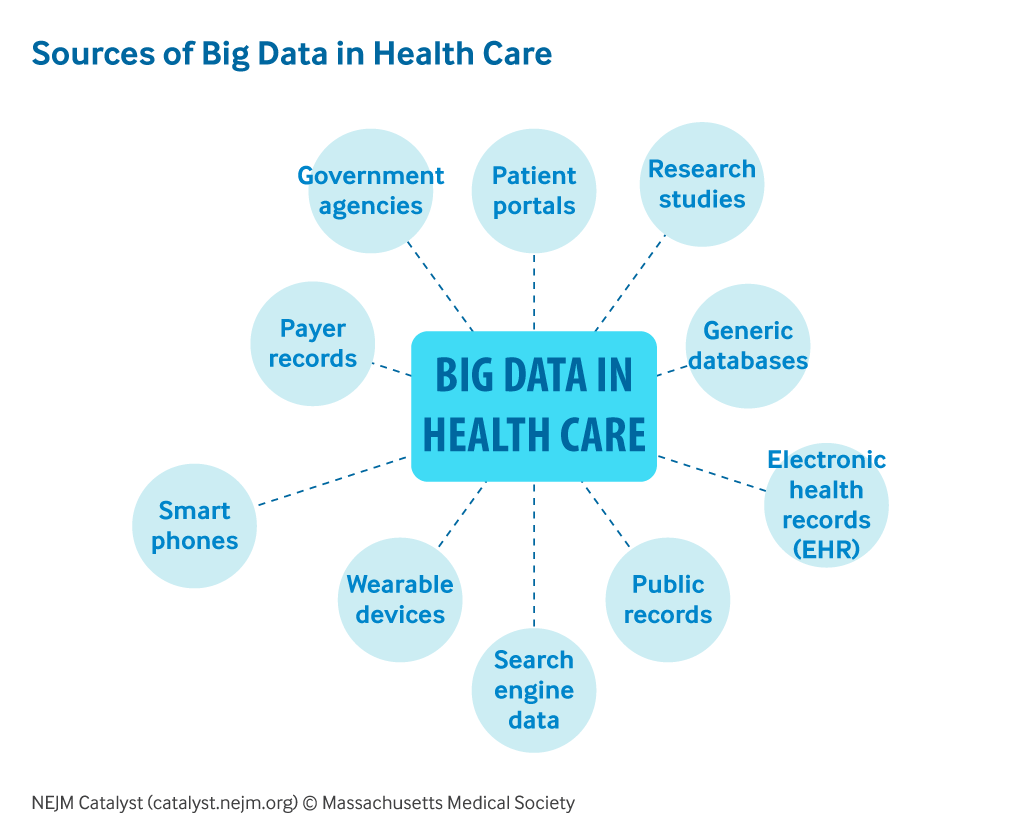
\includegraphics[width=0.75\linewidth,height=0.25\textheight]{images/big-data-healthcare} 

}

\caption{Big Data in Healthcare}\label{fig:sample-fig}
\end{figure}

\hypertarget{introduction}{%
\section{Introduction}\label{introduction}}

It has been estimated that roughly 80\% of health care data is
unstructured data, which can come in the form of videos, sensor data,
images, or text. Although hospitals and researchers used to have a hard
time extracting insights from this type of data, with the recent
advances that have been made in data science and handling big data, this
has created new application areas within the health care industry in
sectors such as genomics, drug trials, predicting patient health, and
medical imagery. Medical imaging research in particular has made
significant progress recently with researchers being able to use
different machine learning algorithms to detect different types of
lesions and cancers from CT and other types of scans. In particular the
advancements of convolutional neural networks to identify whether or not
someone has pneumonia has become extremely promising and can be used to
potentially help doctors identify whether or not someone has pneumonia
that they might have missed, and reduce the amount of hours and amount
of expertise required to view CT scans.

When working with medical imagery data sets though one of the first
problems someone may run into is how to process and handle these large
data sets. When trying to perform analysis on small and medium sized
data sets within R, one would rarely run into complications that would
be attributed to how R is loading and dealing with the data itself. But
what happens when one moves from the world of medium sized data to the
world of Big Data and large data sets? While many of us have probably
been able to read in and load our data for projects into the R Studio
environment without issues and without having to worry about whether the
entirety of our data can even be loaded in, one may begin to run into
complications the larger the data set becomes. By default, R loads all
data into memory and while memory size depends slightly on your
computer's configuration settings under any circumstances one cant have
more than 2,147,483,647 rows or columns, which is roughly equivalent to
2 GB of memory that R is using. (see
\url{http://www.columbia.edu/~sjm2186/EPIC_R/EPIC_R_BigData.pdf}). If
you do end up crossing into the threshold where R can no longer store
all the data in an effective way, there are multiple potential solutions
in the forms of choosing random subsets of the data, buying a computer
with larger memory, or use parallelization and using multiple clusters
to perform the analysis. It is this solution of choosing random subsets
of data, using the keras and tensorflow R packages, that will allow me
to work with and convert large files of image data into a form that
models can be trained on them.

On top of the issue of trying to run analysis on large data sets in R
itself, is the issue of how to best store and load the original
information and data. Often data sets are small enough that they can be
stored on your local computer in a folder that is then uploaded into the
R Studio Environment itself, but what should one do as the size of the
data set substantially increases and one no longer wants to store large
data sets directly on their machine. One solution to this problem is to
take advantage of a cloud computing service and store the data directly
in the cloud, freeing up space and memory on your personal computer. By
storing the data on a cloud computing service, this can become
especially useful when a project begins to get scaled up whether that is
through adding new members to work on the project or when more and more
data gets added to the project. In this project I will take advantage of
Google Cloud Storage to store my data, which will look and store my data
on the cloud without having to take up any space on my local machine.

By combining Google Cloud Storage with Keras and Tensorflow, this will
allow me to utilize a large data set that consisting of medical images.
This data set will then be used to train and create a convolutional
neural networks that will try to identify whether or not someone has
pneumonia from the images.

This project will allow me to answer the questions of what is the best
way to store large data sets and perform computationally expensive
analysis on those data sets? How does one handle and process images so
that analysis can be performed on them, and how effective are
convolutional neural networks at identifying pneumonia within CT scans?

\hypertarget{google-cloud-storage}{%
\section{Google Cloud Storage}\label{google-cloud-storage}}

When trying to work with Big Data, one of the first questions one has to
answer is what is the best way to store and access this data. While
smaller files can be stored directly on your computer and eventually
loaded into R Studio to perform analysis on, when data moves into the
gigabyte, terabyte, or even petabyte range one may not not want to store
this data directly on their machine and use of large chunks of their
limited memory that is available. With the advancement of cloud service
solutions in recent years though, one can now use a platform such as
Google Cloud Platform, Amazon Web Services, or Microsoft Azure, people
can store large amounts of data directly on these platforms and take
advantage of these companies large data warehouses for a small cost.
This can allow one to free up space and memory on their own personal
machine and access the data directly from these servers whenever they
desire.

For this project, I am going to focus on how to setup and store medical
imagery in Google Cloud Storage and learn how this can be connected to R
Studio so that I can then before analysis on these images. The data set
I will be working with is labeled Chest X-Ray images
(\url{https://data.mendeley.com/datasets/rscbjbr9sj/2}) which will be
used to detect and classify whether or not someone has pneumonia. This
data set is roughly 2 GB in size and contains CT scans of patients who
either have or dont have pneumonia. Due to Github having maximum storage
limit of 1 GB, I wanted to look into ways that would allow me to work
with a data set of this size and not have to upload the data directly
into Github itself. One of the solutions for this was to use Google
Cloud Storage and take advantage of the free credits that Google offers
for new users using their service. By uploading and storing the data set
directly onto the Google platform, this meant I could delete the data
set off my computer for the time being and free up memory space.

\begin{figure}

{\centering 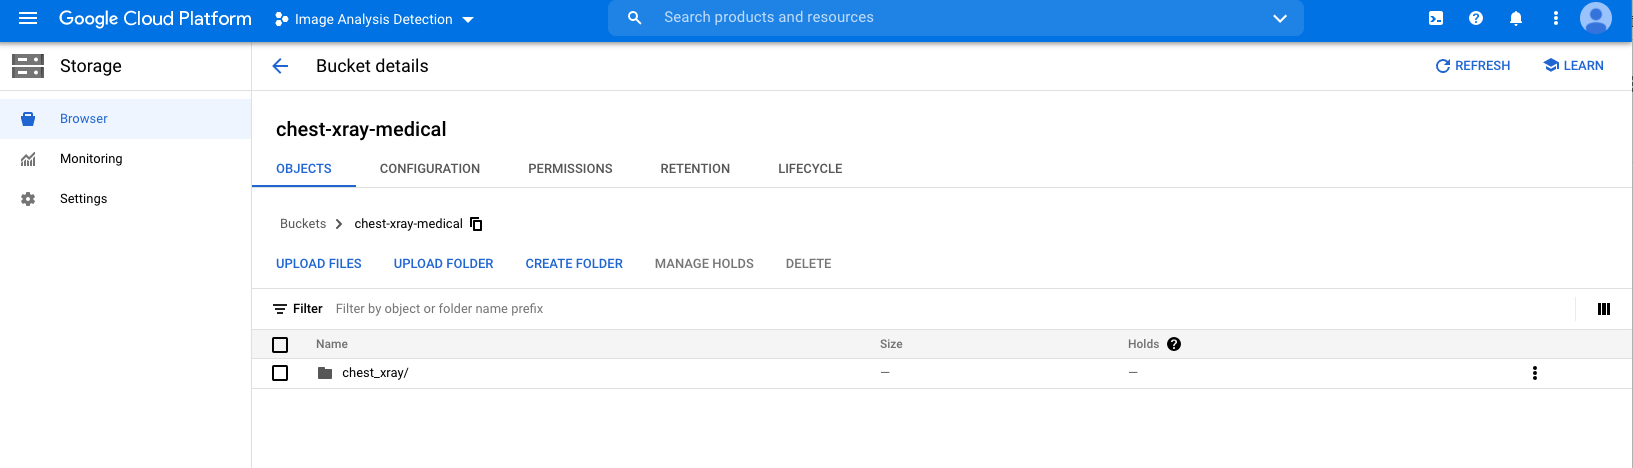
\includegraphics[width=0.75\linewidth,height=0.25\textheight]{images/cloud_storage} 

}

\caption{Google Cloud Storage Platform}\label{fig:sample-fig2}
\end{figure}

In order to actually work with this data in R Studio though, a
connection between R and Google Cloud was required to be setup. By
utilizing the \emph{googleCloudStorageR} package, I was able to setup a
connection that allowed me to download the data from my Cloud Storage
bucket and onto my desktop where it could then be read into R Studio
without having to store the files themselves within R Studio. This
allowed me to not have to store the data in my actual Github repository
but still be able to perform analysis and build models on the images.

\hypertarget{image-transformation-and-tensorflow}{%
\section{Image Transformation and
Tensorflow}\label{image-transformation-and-tensorflow}}

Once the images are in a place where they could be loaded into R, one
needs to put the images into a format where R can actually perform
analysis on them. For images, this can consist of different image
transformations and adjustments such as cropping, brightness,
contrasting, changing the color scale, or resizing an image. This sort
of data augmentation, when performed on all the images in the data set
can help create a more consistent form between all the images. By
putting all the images in grayscale or cropping photos, this makes all
the images' underlying form more consistent and makes it easier for
models to distinguish differences in the images themselves. For the
images in my medical imagery data set, this primarily consisted of
resizing the images on a pixel by pixel basis so they were all the same
size, and then converted them to a grayscale color. This made the
underlying structure of the images the same for all the images in the
dataset.

\begin{figure}

{\centering 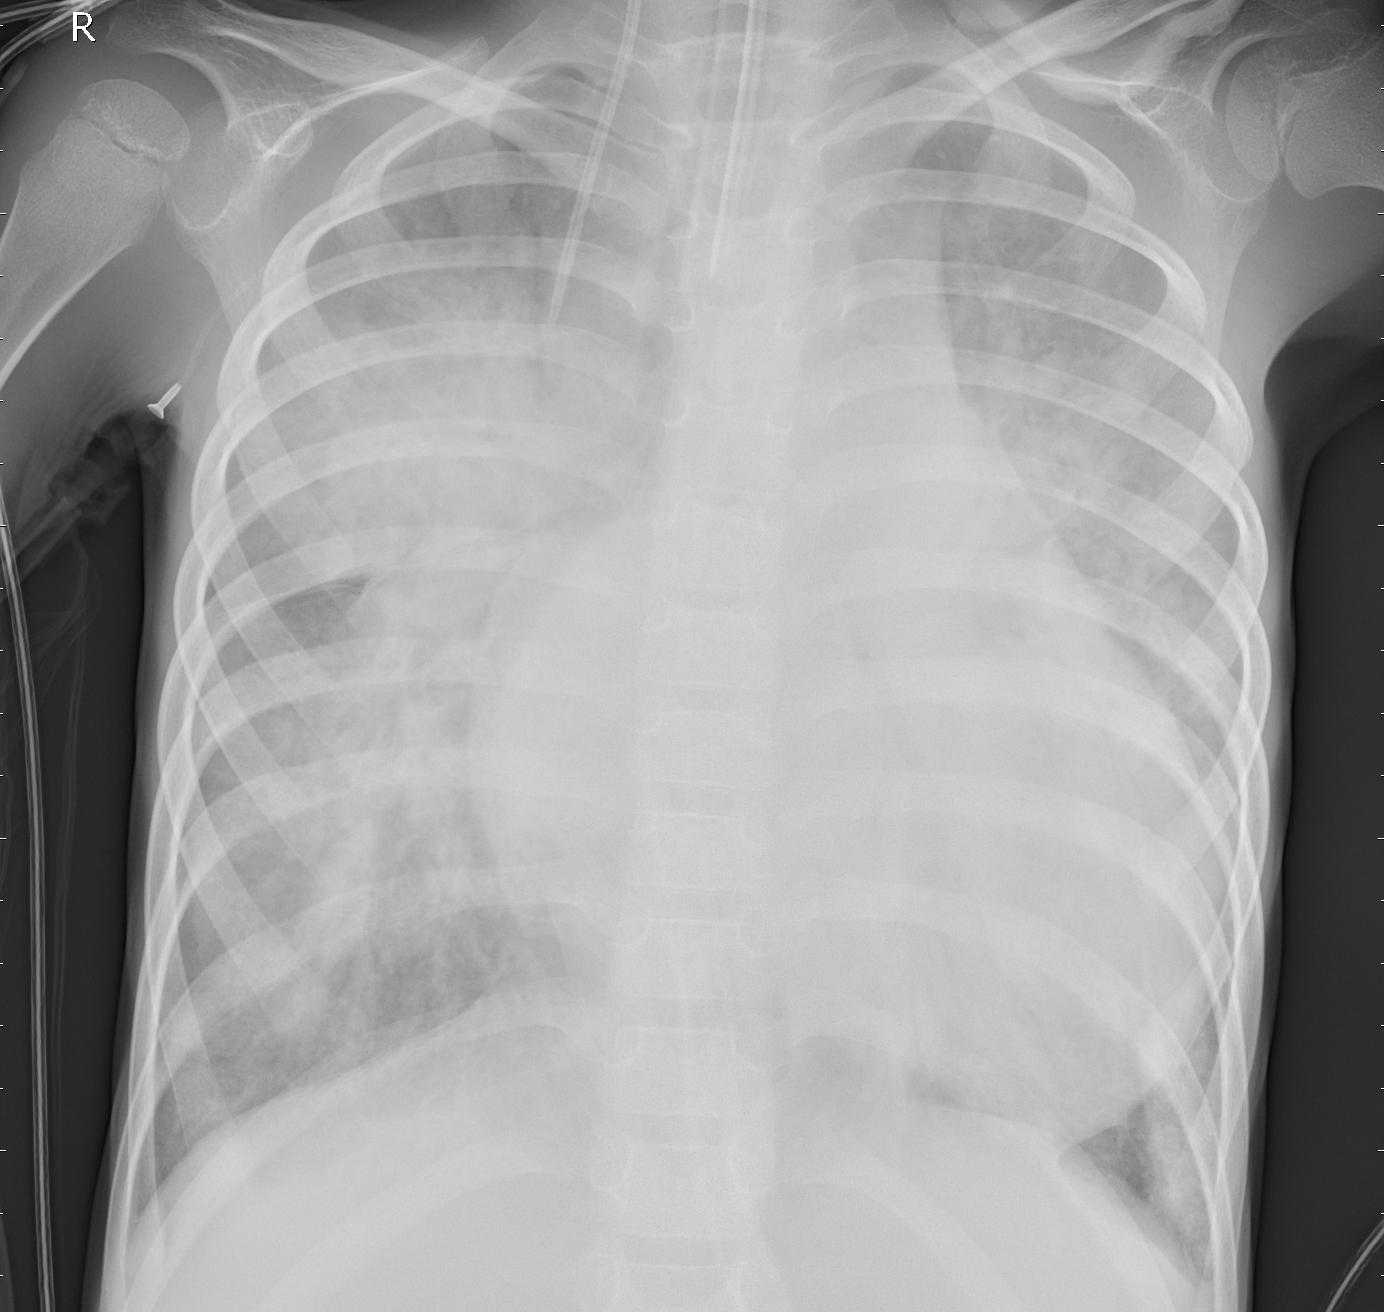
\includegraphics[width=0.75\linewidth,height=0.25\textheight]{images/pneumonia} 

}

\caption{Pneumonia}\label{fig:sample-fig3}
\end{figure}

\begin{figure}

{\centering 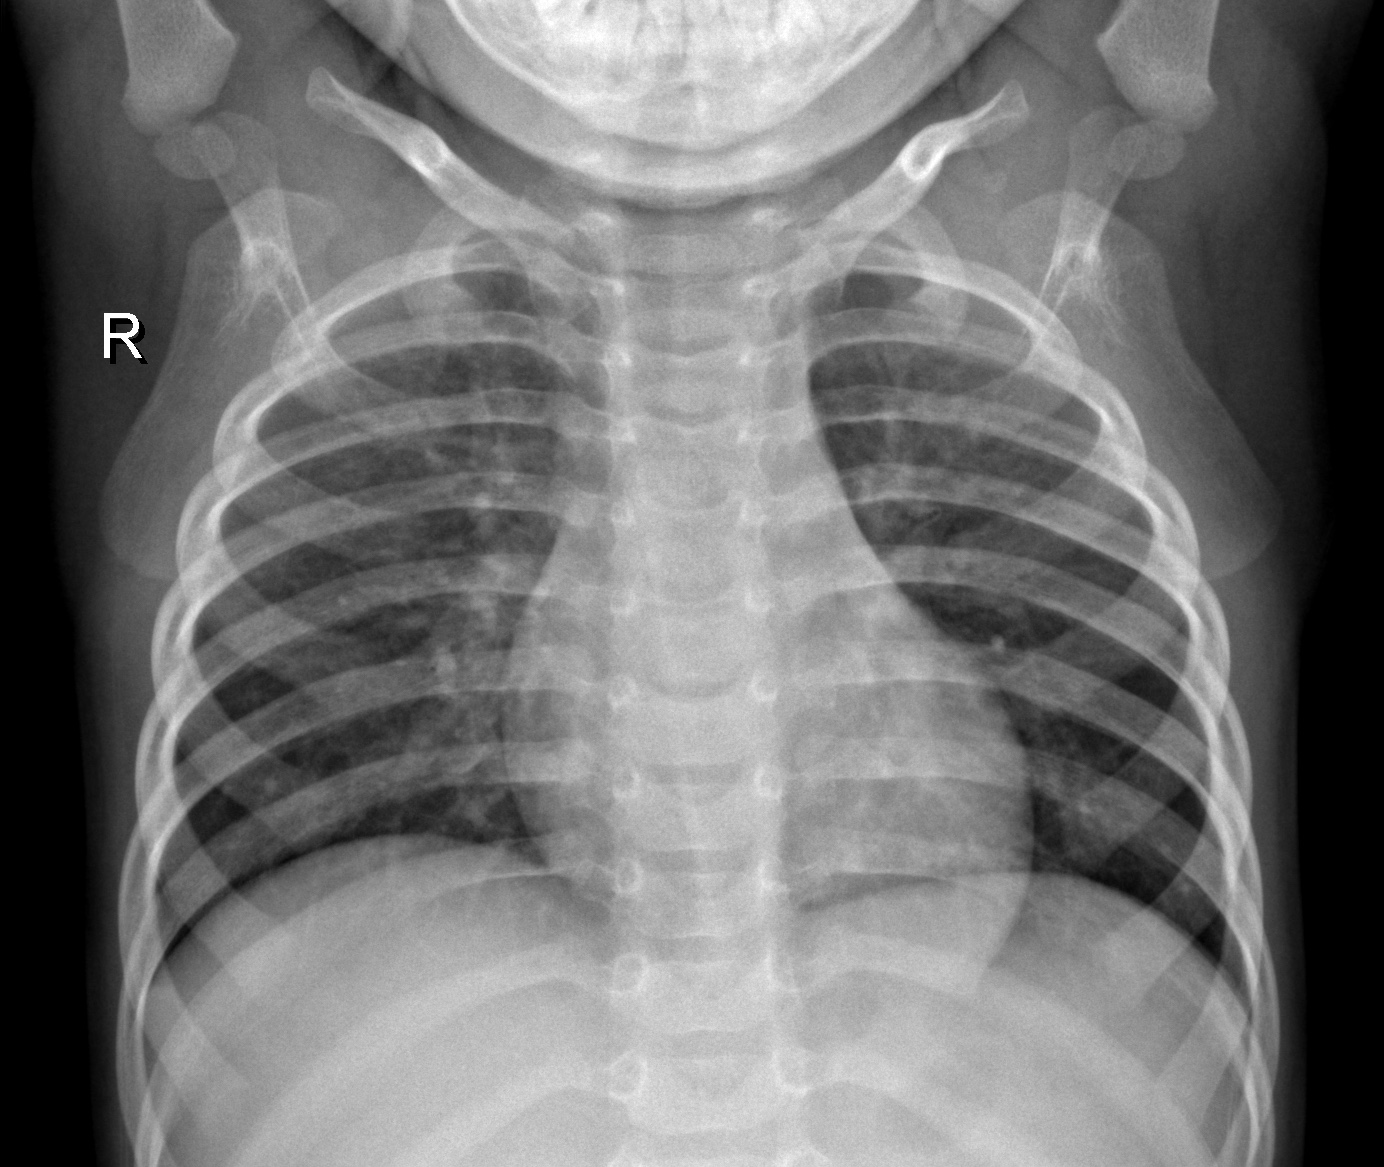
\includegraphics[width=0.75\linewidth,height=0.25\textheight]{images/normal} 

}

\caption{Normal}\label{fig:sample-fig4}
\end{figure}

After getting all the images into the same structure, I needed to
convert them to a form where I could actually perform analysis on the
images. In order to do this I relied on the \emph{tensorflow} R
packages. Tensorflow is a ``scalable and multiplatform programming
interface for implementing and running machine learning
algorithms''(Book page 427). Tensorflow allows execution on both CPU's
and GPU's which help speed up processing time on complicated algorithms.
This package is built around a ``computation graph composed as a set of
nodes where each node represents an operation that may have zero or more
input or output. A tensor is created as a symbolic handle to refer to
the input and output of these operations'' (428 book). A tensor is best
understood as either a scalar, vector , matrices and so on, which all
correspond to a different rank tensor (see image below). These tensors
are created from the values in the data you are working with and then
are used to build and create the complex models one wants to work with

\begin{figure}

{\centering 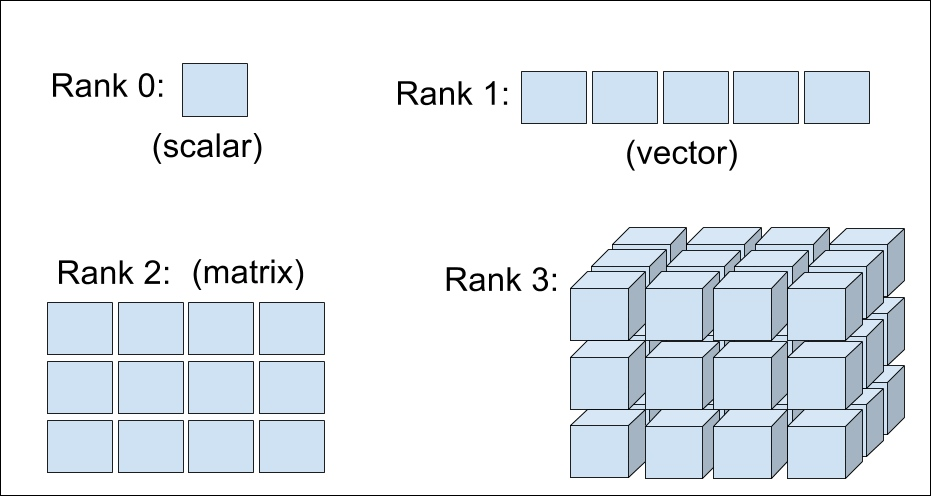
\includegraphics[width=0.75\linewidth,height=0.25\textheight]{images/tensors} 

}

\caption{Tensors in Tensorflow}\label{fig:sample-fig5}
\end{figure}

For the images in my data set, by using Tensorflow I was able to convert
the images into a set of tensors that represented the pixels of the
images themselves. Since the images had been resized to a 32x32 picture
in grayscale coloring, this became a 32x32x1 tensor for each image.
These tensors were then combined with their appropriate label for the
type of image they were, either Normal or Pneumonia, creating a nicely
formatted data set where we could then start to create models to best
classify the data.

\hypertarget{keras-and-convolutional-neural-networks}{%
\section{Keras and Convolutional Neural
Networks}\label{keras-and-convolutional-neural-networks}}

As we could see from the prior pictures of someone who had pneumonia
versus someone who did not have pneumonia, it can be very hard to
discern whether or not someone has pneumonia for a person without the
technical training and expertise to identify pictures of pneumonia from
looking at the CT scans. This ultimately requires doctors and those with
the expertise to spend more time looking at the scans, rather than
spending their already limited time directly helping patients. One way
to help doctors to get back to directly helping patients is by utilizing
machine learning to identify and detect different diseases or ailments
within CT scans. By training and creating models that are able to
discern between a normal or healthy scan versus someone who has a lesion
or has pneumonia, we can begin to use artificial intelligence to
alleviate some of the extraneous work that doctors are required to do.

\hypertarget{keras}{%
\subsection{Keras}\label{keras}}

For this project, I was specifically focused on creating a model that
would would be able to discern between someone who has pneumonia versus
someone who does not have pneumonia. In order to do this I utilized the
\emph{keras} package in order to build a convolutional neural network to
be able to distinguish between the two different diagnosis. Keras is a
``high-level neural network API that is built to run off other libraries
such as Tensorflow to provide a user-friendly interface to building
complex models'' (book page 451). Keras, when working with Tensorflow,
helps to provide the framework to begin building complex neural network
models. This package will allow me to be able to not only train and
build the model, but be able to test the model on another subset of
images and be able to begin to predict whether or not someone has
pneumonia from looking at a specific image. Specifically I used the
keras package to build out a convolutional neural network that have been
shown to work extremely well for image classification tasks.

\hypertarget{neural-networks}{%
\subsection{Neural Networks}\label{neural-networks}}

Convolutional Neural Networks (CNN) at a high level are a form of deep
learning thattakes an image as an input and eventually classifies it
under a certain category. These types of networks are used heavily to
perform tasks such as facial recognition, object detection, and image
classification to just list a few. CNN's are a specific type of neural
network, which falls under the branch of machine learning called deep
learning. Neural networks are extremely popular today due to recent
advances in both the algorithms for the models and the computer
architecture which allows for much faster processing times of these
complex models.

\begin{figure}

{\centering 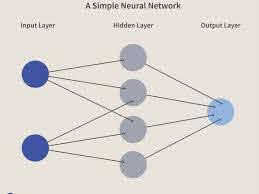
\includegraphics[width=0.75\linewidth,height=0.25\textheight]{images/neural_net} 

}

\caption{Neural Network example}\label{fig:sample-fig6}
\end{figure}

This figure above shows an example of what the underlying structure of a
neural network looks like (see figure 6, ADD Source). The neural network
show in this example consists of one input layer, one hidden layer with
4 hidden units, and then one output layer. The input layer would be the
exact data you are feeding into the model, so for this picture this
would mean there was two examples being fed into network to train the
model. Then we can see how each of the input layers are connected to
three of the gray nodes in the hidden layer. While this model only has
one hidden layer and the inputs are only connected to 3 of the hidden
units, in other models one could create multiple hidden layers, each
with a different number of hidden units, and the number of units that
are connected together from layer to layer can vary as well. After that
we can see that there is one output layer for this example, but other
networks can contain varying numbers of output units as well. Neural
networks in general can contain differing number of hidden layers,
hidden units, input and output units and vary based on the data they
have and the problem they are trying to solve. In general data is fed
into the model, it is passed through the network using weights, and then
often trained using a technique called backwards propagation. This
technique is able to optimize the model by comparing the result found by
the model to the true results, and then working backwards through the
model to update the weights so that the model can better classify the
input data. Neural networks in general have been shown to be extremely
successful at a broad range of tasks such as natural language processing
to self-driving cars and everything inbetween.

\hypertarget{convolutional-neural-networks-cnn}{%
\subsection{Convolutional Neural Networks
(CNN)}\label{convolutional-neural-networks-cnn}}

As mentioned earlier, CNN's a specific form of Neural Network that is
based heavily on how the visual cortext of the human brain works when
recogizing images, which is what allows it to perform extremely well on
image classification tasks. At a high level CNN's work by ``combining
the low level features in a layer-wise fashion to form high-level
features'' (book 519). So rather than just looking at each pixel of an
image separately, this model works to combine pixels into distinct
features that can then be used to identify exact objects within the
images. In order for the model to actual identify distinct features it
relies on an idea called feature mapping that groups patches of pixels
together in the image and combines them into one feature in the new
feature map. This is based on the underlying assumption that in the
context of image data, ``nearby pixels are typically more relevant to
each other than picels that are far away from each other'' (book 520).

In order to actually perform this feature mapping though a CNN relies on
creating a series of different types of layers in the form of
convolution layers, subsampling layers, pooling layers, and dropout
layers.

\hypertarget{convolution-layers}{%
\subsubsection{Convolution layers}\label{convolution-layers}}

Convolution layers is one of the first layers that begins extracting
features from the input images. This layer works by taking an input
matrix that represents the image and a filter matrix, of potentially a
different size, with a set of weifhts. These two matrices are multiplied
together to create a feature map that begins to identify the low level
features such as edges, blurriness, or sharpness of the image.

\hypertarget{subsampling-and-pooling-layers}{%
\subsubsection{Subsampling and Pooling
Layers}\label{subsampling-and-pooling-layers}}

Another type of key layer is the subsampling and pooling layers. Usually
the feature map that is created from the previous convolution layer is
then fed into a subsampling/pooling layer. These layers work by
combining small subsections of the feature map in order to simplify the
feature map. The advantages of this include leading to higher
computational efficiency by decreasing the size of the features and the
number of parameters that are required to learn, as well as introducing
local invariance that helps to generate feature that are more robust to
noise from the input images
(\url{https://www.mathworks.com/discovery/convolutional-neural-network-matlab.html}).

\hypertarget{dropout-layers}{%
\subsubsection{Dropout layers}\label{dropout-layers}}

Dropout layers are then used to prevent over-fitting of the data set. It
can be very easy to create a CNN that gets over-trained but then fails
to perform well on the testing set of data. To prevent over-fitting and
make the model work well for a broader range of images for general
performance, dropout layers are introduced as a form of regularization.
Dropout is usually applied to hidden units of layers and works by
``during the training phase of a neural network, a fraction of the
hidden units are randomly dropped at every iteration. This dropping out
of random units requires the remaining units to rescale to account for
the missing units which forces the network to learn a redundant
representation of the data'' (book 537). This makes it so the model is
more generalizable and robust to changes in patterns in the data and
prevent overfitting.

\hypertarget{challenges}{%
\subsubsection{Challenges}\label{challenges}}

When working with CNN's, these different types of layers that the
network can be built off can all be included multiple times and in
different orders. For example one could create a network of just a
convolution layer and a dropout layer or someone could create a model
that is convolution layer, pooling layer, convolution layer, and then
two dropout layers. There is no set rules around what order or how many
different layers your network can have. On top of having unlimited
variations of the type of layers within the network, there is also
unlimited parameters that one can choose in terms of the size of the
feature map, the number of units to pool together in the pooling layer,
or the number of units to dropout in the dropout layer to just list a
few examples. Due to having so many input parameters that can be changed
and altered when it comes to building the model, finding the best
possible input parameters and underlying structure of the model can
become computationally expensive very quickly.

On top of CNN's being very computationally expensive to run, being able
to interpret the outputs and inputs of individual layers of the network
is its own separate issue. Often these types of models are referred to
as ``black box'' models because while a human can understand the input
and outputs of the models, it is often hard to decipher and understand
what exactly the model is doing inside the box. While there has been
promising developments in this area such as Visualizing Activation
Layers (add a link ) and Occlusion Sensitivity (add a link) , this still
remains an area of the field that a lot of future work can be done in.
So while CNN's have been shown to do an incredible job at image
classification tasks, optimizing and understanding these types of models
is an area that can cause problems and issues.

\hypertarget{cnns-with-medical-images}{%
\subsection{CNN's with Medical Images}\label{cnns-with-medical-images}}

For my project, I wanted to use Convolutional Neural Networks to see how
well this type of network could perform on the task of trying to
classify whether or not someone had pneumonia based just of a CT scan.
At this point I have already gotten my images into a form that allows
them to be passed as inputs to build a model, so the next step was for
me to begin training the model.

\hypertarget{come-back-and-describe-this}{%
\paragraph{come back and describe
this}\label{come-back-and-describe-this}}

I first started off by having my data split into training, validation,
and testing sets. The training set would be used to train the model, the

\hypertarget{put-in-an-image-that-shows-the-original-split-in-the-data}{%
\subparagraph{put in an image that shows the original split in the
data}\label{put-in-an-image-that-shows-the-original-split-in-the-data}}

\hypertarget{future-work}{%
\section{Future Work}\label{future-work}}

\begin{itemize}
\tightlist
\item
  working with google cloud platform environment, not having to store
  the data on my computer at all -model could have been optimized
\item
  further application areas, such as lesions and other things that can
  be detected in ct scans (enhancing images
  themself)\url{https://healthitanalytics.com/news/deep-learning-model-can-enhance-standard-ct-scan-technology}
\end{itemize}

\bibliographystyle{agsm}
\bibliography{bibliography.bib}

\end{document}
